\documentclass{article}

% if you need to pass options to natbib, use, e.g.:
%     \PassOptionsToPackage{numbers, compress}{natbib}
% before loading neurips_2020

% ready for submission
% \usepackage{neurips_2020}

% to compile a preprint version, e.g., for submission to arXiv, add add the
% [preprint] option:
% \usepackage[preprint]{neurips_2020}

% to compile a camera-ready version, add the [final] option, e.g.:
\usepackage[final]{neurips_2020}

% to avoid loading the natbib package, add option nonatbib:
% \usepackage[nonatbib]{neurips_2020}

\usepackage[utf8]{inputenc} % allow utf-8 input
\usepackage[T1]{fontenc}    % use 8-bit T1 fonts
\usepackage{hyperref}       % hyperlinks
\usepackage{url}            % simple URL typesetting
\usepackage{booktabs}       % professional-quality tables
\usepackage{amsfonts}       % blackboard math symbols
\usepackage{nicefrac}       % compact symbols for 1/2, etc.
\usepackage{microtype}      % microtypography
\usepackage{xcolor}
\usepackage{media9}
\usepackage{float}
\usepackage{graphicx}
\usepackage{blindtext}
\usepackage{subcaption}

\title{A Transformer-Based Generative Model for Efficient and Specific CRISPR gRNA Design}

\author{
  \makebox[\linewidth]{%
  \normalfont
    \begin{tabular}{ccc}
      \textbf{Tien Vu} & \textbf{Daniel Chen} & \textbf{Anton John Del Mar} \\
      Electrical and Computer Engineering & Electrical and Computer Engineering & Electrical and Computer Engineering \\
      University of California, San Diego & University of California, San Diego & University of California, San Diego \\
      \texttt{tqvu@ucsd.edu} & \texttt{dychen@ucsd.edu} & \texttt{adelmar@ucsd.edu}
    \end{tabular}
  }\\[1ex]  
}

\begin{document}

\maketitle

\iffalse
\begin{abstract}
There is a lot of potential health improvements with the development of genome editing through CRISPR-Cas9. CRISPR-Cas9 is a gene-editing tool that uses a guide RNA to direct the Cas9 enzyme to a specific DNA sequence, where it makes a precise cut to modify the gene. In this project we aim to use transformers to generate gRNA's for CRISPR-Cas9 in hopes to develop a method of creating the most effecient gRNA of a given target DNA sequence. 
\end{abstract}
\fi 

\vspace{-2em}

\section{Motivation}
CRISPR-Cas9 is a gene-editing tool that uses a guide RNA (gRNA) to direct the Cas9 enzyme to a specific DNA sequence, where it makes a precise cut to modify the gene. Predictive ranking models are oftentimes used to identify which gRNA sequence in a pre-existing pool will yield the most activity (i.e. effectiveness) at a particular DNA test site \hyperref[Reference 3]{[3]}. However, these pre-existing gRNA pools are typically obtained using rule-based heuristics and empirically validated by researchers \hyperref[Reference 4]{[4]}. Thus, the input pool may fail to capture other possible high-efficiency gRNAs that fall outside of these rules. With that said, having a model that can generate new gRNA sequences and score them can provide greater insight for researchers to determine if they already have an optimal gRNA sequence or if there are better options they can test. Our paper will investigate the possible advantages of this approach, particularly its ability to accelerate optimal gRNA discovery with scored sequences. This expands the existing search pool and helps researchers identify gRNA sequences with higher predicted activity for a given DNA target site.

\begin{figure}[H]
    \centering
    \begin{minipage}{0.32\textwidth}
        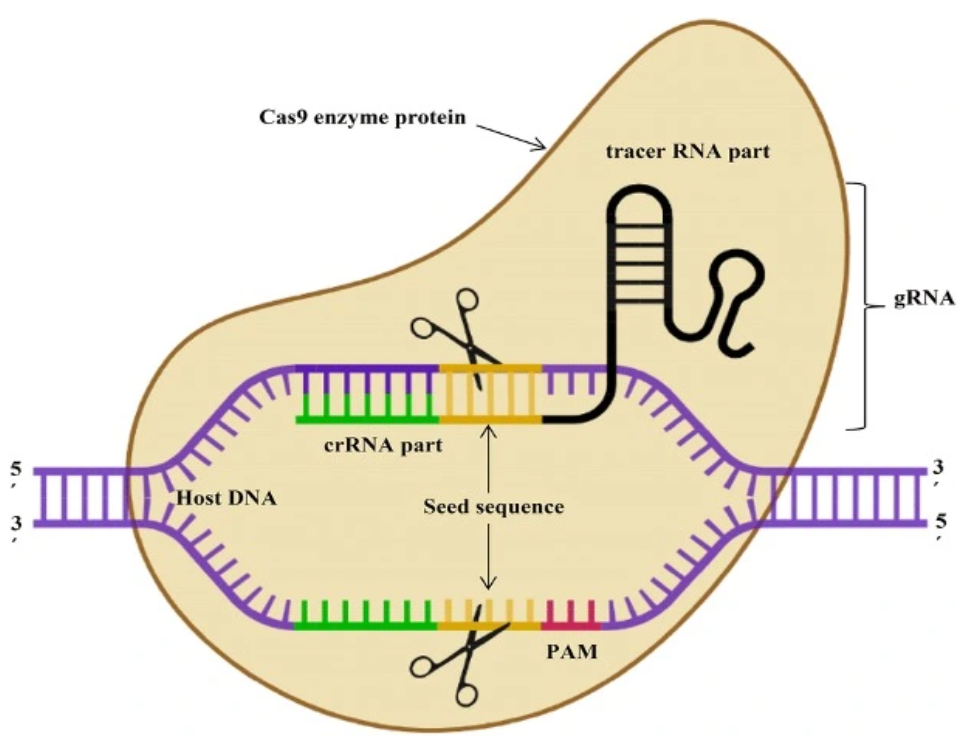
\includegraphics[width=\linewidth]{Pictures/CRISPR_Cas9.png} 
    \end{minipage}
    \caption{CRISPR-Cas9 system is a monomeric protein consisting of a single Cas9 enzyme that makes a complex with a guide RNA (gRNA) \hyperref[Reference 10]{[10]}} 
\end{figure}

\vspace{-1em}

\section{Problem}
Gene editing remains at the forefront of modern biomedical research, holding immense potential for the treatment of unique genetic disorders and complex diseases. Of these technologies, CRISPR-Cas9 is a widely-used approach that relies on gRNA to direct Cas9 enzymes to a target DNA site for precise genomic modifications \hyperref[Reference 5]{[5]}. The accuracy and effectiveness of CRISPR-Cas9 heavily depends upon the construction of the gRNA, such that it closely matches the target sequence to maximize on-target activity while minimizing off-target edits \hyperref[Reference 6]{[6]}. However, gRNA design is a non-trivial optimization problem that must balance tightly-coupled biological factors, such as PAM compatibility, sequence features, genomic location, and self-complementarity \hyperref[Reference 6]{[6]}\hyperref[Reference 8]{[8]}\hyperref[Reference 11]{[11]}. In this context, deep generative models stand out as an opportunity to synthesize optimal gRNA sequences given an input target DNA sequence.  


\section{Related Works}
Although CRISPR was first discovered in 1987, it was not until 2012 that Nobel Laureates Jennifer Doudna and Emmanuelle Charpentier discovered the use of the CRISPR-Cas9 system in precise gene editing \hyperref[Reference 5]{[5]}. Despite the relative novelty of this technology, research in improving CRISPR-Cas9 is ever expanding. This includes predictive ranking models that score existing gRNA efficiency based on a target sequence and contextual features, heuristic rule-based models that generate gRNAs without deep learning, and existing generative models that are still at their infancy. However, each of these approaches all have their limitations which we aim to address with our approach. Rankers are trained on data of gRNA that have been tested and bound to Cas9 and how well they perform at the reaching their target \hyperref[Reference 7]{[7]}. They may face biases in their ranking, favouring gRNA similar to their training set. Relative rankers are also limited to only scoring existing gRNA performance, but it cannot generate the gRNA itself and needs users to find their own sequences to test on. If a user were to generate gRNAs that are based on poor assumptions, a ranking model will still output a best performing gRNA despite all of them being from a suboptimal pool \hyperref[Reference 7]{[7]}. Existing heuristic models such as CHOPCHOP are limited by the rules researchers know for generating gRNA but may be missing features and patterns that can be learned by deep learning models \hyperref[Reference 7]{[7]}\hyperref[Reference 6]{[6]}. A hybrid of a heuristic rule-based and a deep generative model could improve both shortcomings. Lastly, deep generative models such as DeepGuide are currently limited to narrow target organisms such as \textit{Yarrowia lipolytica} and are not widely adopted by researchers yet \hyperref[Reference 2]{[2]}. Our approach intends to combine the advantages of seemingly different approaches to address their respective limitations.


\section{Proposed Solution}
For this project, we will be implementing a transformer architecture along with a dataset containing a DNA with its most effective gRNA pair. Transformers perform better in natural language processing because of their self-attention ability, unlike recurrent neural networks (RNN) and long short-term memory (LSTM) models. This makes transformers the most ideal candidate for our genomic processing problem. For the encoder, we take an input sequence and pass it through multiple feedforward and self-attention layers, where the final output of the encoder is a representation of the input sequence \hyperref[Reference 9]{[9]}. In our case, we would pass in a DNA sequence and the self-attention mechanism of the transformer will identify which parts of the DNA are important in generating the corresponding gRNA by recognizing patterns and motifs that humans may not be able to comprehend. The decoder should output the most effective gRNA sequence given the patterns it learned between DNA and the effective gRNA. It does this by using cross attention to prioritize relevant parts of the relationship between a DNA and the effective gRNA sequence \hyperref[Reference 9]{[9]}. To penalize the model, we came up with an unconventional way to calculate loss: we will use a gRNA ranker! With the ranker, we can calculate the corresponding loss with the effectiveness score of the generated gRNA. gRNA generative models are limited by their sample size and downstream validation, meaning it is not easily experimental confirmed. In contrast, gRNA rankers are limited by the finite pool of existing gRNA sequences, meaning it only ranks without generating new sequences. Our solution addresses the critical shortcomings of these two major existing solutions by generating multiple educated predictions of gRNA’s given a DNA target sequence and is then processed through an existing ranker in order to determine the best of the generated gRNA sequences \hyperref[Reference 2]{[2]}. We can validate our generated gRNA's performance by comparing it against existing gRNA sequences targeting the same DNA sequence. Therefore, if our generative results cannot outperform the existing solution, that means the existing solution is already a good or optimal performer.


\section{Project Timeline}
During week 4, we will focus on finding an appropriate dataset, preferably one with a DNA-gRNA pairing. We have already found a gRNA ranker model, CRISPRon, to be able to test the efficiency of our generated gRNA sequences. During weeks 5-6, we will work on the actual development of the transformer model, ensuring we have the proper structure and strong code base. For the upcoming weeks 7-8, we will train our model with the dataset we find and make sure that the generated gRNA sequences are logical, tweaking parameters as needed. For our final push during weeks 9-10, we will test the effectiveness of our output gRNA using the predictive ranking model. Hopefully our generator is able to output even more effective gRNA sequences for the final project!

\newpage

\section*{References}

\small
\label{Reference 1} [1] Anthon, Christian et al. “CRISPRon/off: CRISPR/Cas9 on- and off-target gRNA design.” Bioinformatics (Oxford, England) vol. 38,24 (2022): 5437-5439. doi:10.1093/bioinformatics/btac697 

\label{Reference 2} [2] Baisya, D., Ramesh, A., Schwartz, C. et al. Genome-wide functional screens enable the prediction of high activity CRISPR-Cas9 and -Cas12a guides in Yarrowia lipolytica. Nat Commun 13, 922 (2022). https://doi.org/10.1038/s41467-022-28540-0

\label{Reference 3} [3] Chuai, G., Ma, H., Yan, J. et al. DeepCRISPR: optimized CRISPR guide RNA design by deep learning. Genome Biol 19, 80 (2018). https://doi.org/10.1186/s13059-018-1459-4

\label{Reference 4} [4] Haeussler, M., Schönig, K., Eckert, H. et al. Evaluation of off-target and on-target scoring algorithms and integration into the guide RNA selection tool CRISPOR. Genome Biol 17, 148 (2016). https://doi.org/10.1186/s13059-016-1012-2

\label{Reference 5} [5] Jinek, Martin et al. “A programmable dual-RNA-guided DNA endonuclease in adaptive bacterial immunity.” Science (New York, N.Y.) vol. 337,6096 (2012): 816-21. doi:10.1126/science.1225829

\label{Reference 6} [6] Kornel Labun, Tessa G Montague, Maximilian Krause, Yamila N Torres Cleuren, Håkon Tjeldnes, Eivind Valen, CHOPCHOP v3: expanding the CRISPR web toolbox beyond genome editing, Nucleic Acids Research, Volume 47, Issue W1, 02 July 2019, Pages W171–W174, https://doi.org/10.1093/nar/gkz365

\label{Reference 7} [7] Xiang, X., Corsi, G.I., Anthon, C. et al. Enhancing CRISPR-Cas9 gRNA efficiency prediction by data integration and deep learning. Nat Commun 12, 3238 (2021). https://doi.org/10.1038/s41467-021-23576-0

\label{Reference 8} [8] Xu H, Xiao T, Chen CH, Li W, Meyer CA, Wu Q, Wu D, Cong L, Zhang F, Liu JS, Brown M, Liu XS. Sequence determinants of improved CRISPR sgRNA design. Genome Res. 2015 Aug;25(8):1147-57. doi: 10.1101/gr.191452.115. Epub 2015 Jun 10. PMID: 26063738; PMCID: PMC4509999. 

\label{Reference 9} [9] Attention Is All You Need, Ashish Vaswani and Noam Shazeer and Niki Parmar and Jakob Uszkoreit and Llion Jones and Aidan N. Gomez and Lukasz Kaiser and Illia Polosukhin, 2023, 1706.03762, arXiv, cs.CL, https://arxiv.org/abs/1706.03762

\label{Reference 10} [10] CRISPR Cas9 Image, https://www.elveflow.com/microfluidic-reviews/crispr-cas9-and-its-relation-with-microfluidics/

\label{Reference 11} [11] Mingkun Luo, Jun Wang, Zaijie Dong, Chenghui Wang, Guoqing Lu, CRISPR-Cas9 sgRNA design and outcome assessment: Bioinformatics tools and aquaculture applications, Aquaculture and Fisheries, Volume 7, Issue 2, 2022, Pages 121-130, ISSN 2468-550X, https://doi.org/10.1016/j.aaf.2021.10.002.

\end{document}